\section{Desarrollo de pruebas de penetración}
\subsection{HTB01 - OpenAdmin}
\subsubsection{Escaneo}
Como inicio de la prueba de penetración se realiza un escaneo de puertos con la herramienta “Nmap”, donde se encuentran dos puertos abiertos, el puerto 22 con el servicio SSH y el puerto 80 con un servidor web Apache.
\begin{figure}[H]
    \centering
    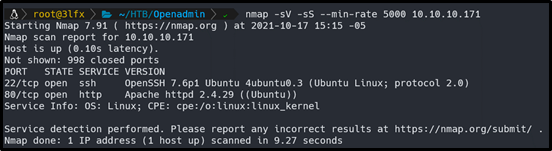
\includegraphics[width=0.99\textwidth]{imagenes/scanopen.png}
    \caption{Escaneo de puertos OpenAdmin}
\end{figure}
\subsubsection{Análisis de vulnerabilidades y debilidades}
Se procedió a revisar el sitio web, teniendo la solo la página predeterminada de Apache.
\begin{figure}[H]
    \centering
    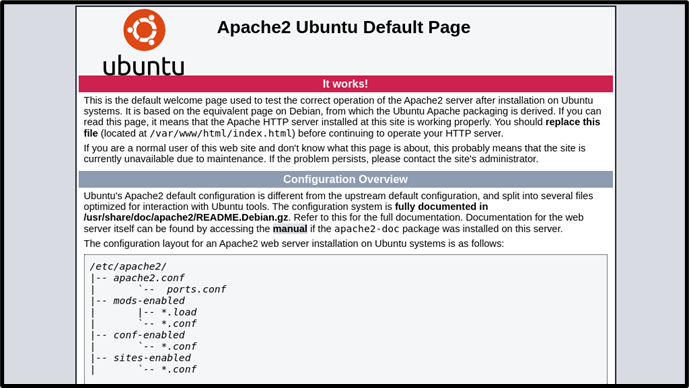
\includegraphics[width=0.99\textwidth]{imagenes/apapred.png}
    \caption{Página web predeterminada de Apache en OpenAdmin}
\end{figure}
Lo siguiente a realizar fue usar la herramienta “Gobuster” para enumerar los directorios del servidor web.

\begin{figure}[H]
    \centering
    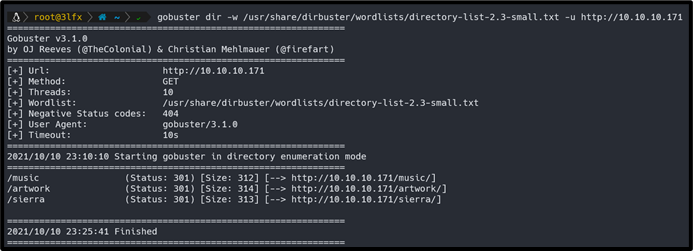
\includegraphics[width=0.99\textwidth]{imagenes/enudicopen.png}
    \caption{Enumeración de directorios en OpenAdmin}
\end{figure}
\par
Del proceso anterior se registró 3 directorios, se procedió a acceder al directorio music donde se encontraba la página SOLMUSIC.

\begin{figure}[H]
    \centering
    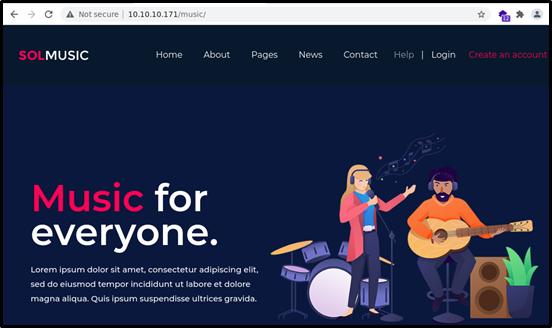
\includegraphics[width=0.99\textwidth]{imagenes/musicopen.png}
    \caption{Página web Music en OpenAdmin}
\end{figure}

Al revisar esta página se descubrió que al dirigirse al Login nos redirige al directorio “ona”. Se observa el uso del servicio OpenNetAdmin con versión 18.1.1 como se muestra en la siguiente imagen.

\begin{figure}[H]
    \centering
    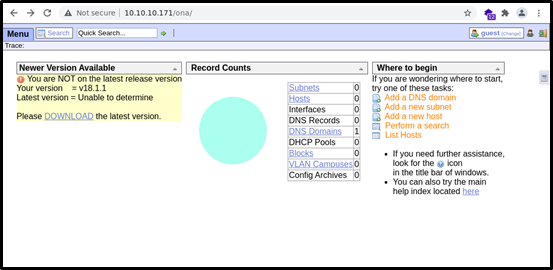
\includegraphics[width=0.99\textwidth]{imagenes/onaopen.png}
    \caption{Servicio OpenNetAdmin}
\end{figure}
Al buscar información sobre la versión de este servicio, se encontró que es vulnerable a ejecución remota de comandos (VU01).

La vulnerabilidad es debido a que la función “ws\_ping”, del módulo “tooltips”, realiza ejecución de código para realizar ping a una dirección IP, mediante el parámetro “form” donde se encontrará la IP esperada por la función utilizada, se puede inyectar comandos de Shell.
\subsubsection{Explotación}
Para la explotar la vulnerabilidad encontrada se utilizó un exploit escrito en Python perteneciente al usuario “amriunix” de GitHub \cite{ona}. Una vez descargado el exploit se ejecutó, obteniendo acceso a la máquina como “www-data”. 
\begin{figure}[H]
    \centering
    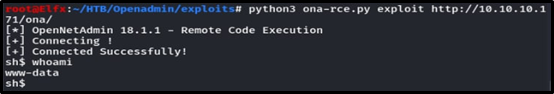
\includegraphics[width=0.99\textwidth]{imagenes/expopen.png}
    \caption{Ejecución de exploit en OpenAdmin}
\end{figure}
\subsubsection{Escalamiento de Privilegios}
Se procede a analizar los directorios con lectura permitida, encontrando el archivo “database\_settings.inc.php”, donde se encontró una contraseña en texto plano que resulta ser del usuario Jimmy (DE01).
\begin{figure}[H]
    \centering
    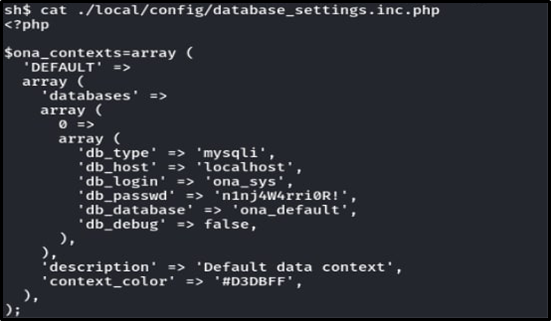
\includegraphics[width=0.8\textwidth]{imagenes/contsql.png}
    \caption{Hallazgo de contraseña en OpenAdmin}
\end{figure}
Una vez teniendo esta contraseña se procede a realizar una conexión mediante el servicio SSH como el usuario Jimmy, donde se consigue el acceso teniendo como prueba la siguiente imagen.
\par
\begin{figure}[H]
    \centering
    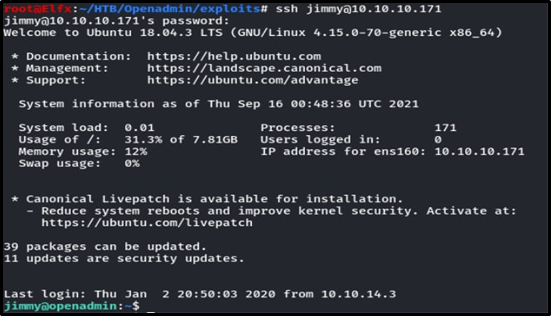
\includegraphics[width=0.8\textwidth]{imagenes/acjim.png}
    \caption{Acceso al usuario Jimmy en OpenAdmin}
\end{figure}

Lo siguiente a realizar es una búsqueda de archivos que nos permitan tener acceso al usuario Joanna. En el directorio “/var/www/internal” se encuentra el archivo “main.php” que al analizarlo se observa la ejecución de lectura del archivo “id\_rsa” perteneciente al usuario Joanna (DE02).
\begin{figure}[H]
    \centering
    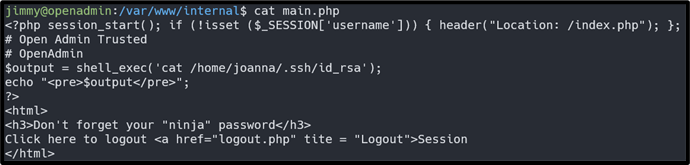
\includegraphics[width=0.99\textwidth]{imagenes/idjoa.png}
    \caption{Archivo de ejecución para lectura de ``id\_rsa" de Joanna}
\end{figure}
Para tener acceso a esta sección no se puede realizar mediante el puerto 80, por ello se revisa los puertos abiertos de la máquina desde adentro mediante netstat.
\begin{figure}[H]
    \centering
    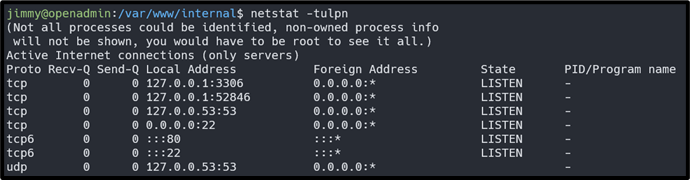
\includegraphics[width=0.99\textwidth]{imagenes/listpa.png}
    \caption{Listado de puertos abiertos internamente en OpenAdmin}
\end{figure}
Del proceso anterior se encuentra el puerto 3306 y 52846, teniendo éxito al realizar la llamada al archivo “main.php” a través del puerto 52846, como prueba de ello se tiene la siguiente imagen.
\begin{figure}[H]
    \centering
    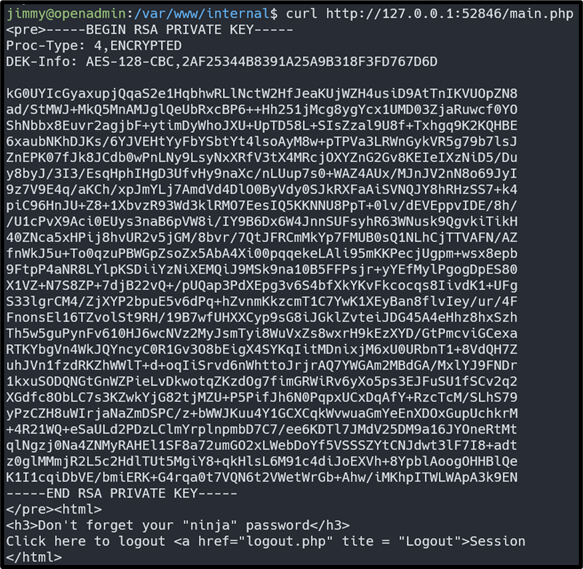
\includegraphics[width=0.58\textwidth]{imagenes/claprjoa.png}
    \caption{Clave privada de Joanna}
\end{figure}
Una vez obtenido la clave privada de Joanna que está protegida por una frase de contraseña como se indica en la imagen anterior, se procede a usar la herramienta “ssh2john” para convertir la clave privada en un hash que pueda ser descifrado con John the Ripper.
\begin{figure}[H]
    \centering
    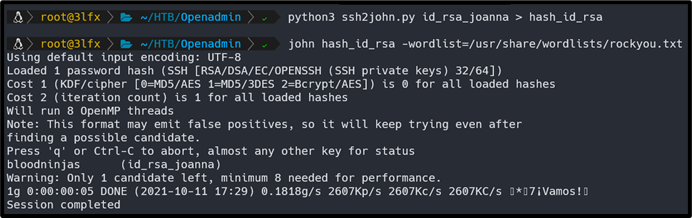
\includegraphics[width=0.99\textwidth]{imagenes/desjoa.png}
    \caption{Descifrado de contraseña de Joanna}
\end{figure}
Como resultado del descifrado se obtuvo que la frase de contraseña es “bloodninjas”. Ahora se puede realizar una conexión ssh a la máquina con el usuario Joanna, teniendo como prueba la siguiente imagen.
\begin{figure}[H]
    \centering
    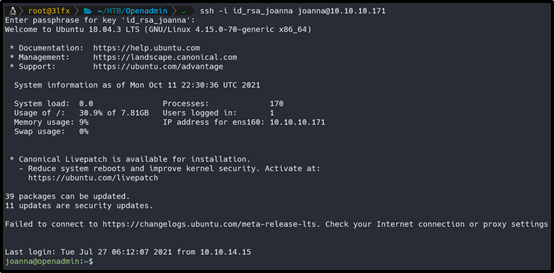
\includegraphics[width=0.99\textwidth]{imagenes/acjoa.png}
    \caption{Acceso al usuario Joanna en OpenAdmin}
\end{figure}
Una vez accedido al usuario Joanna se puede procederá a escalar privilegios a usuario “root”, para ello verificamos que comandos puede ejecutar en la máquina.
\begin{figure}[H]
    \centering
    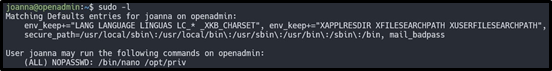
\includegraphics[width=0.99\textwidth]{imagenes/perejop.png}
    \caption{Permiso de ejecución sin contraseña con usuario Joanna}
\end{figure}
Como se muestra en la anterior imagen se puede ejecutar “/bin/nano /opt/priv” sin necesidad de contraseña, al proceder a ejecutarlo se abre nano con el archivo “/opt/priv”.
\begin{figure}[H]
    \centering
    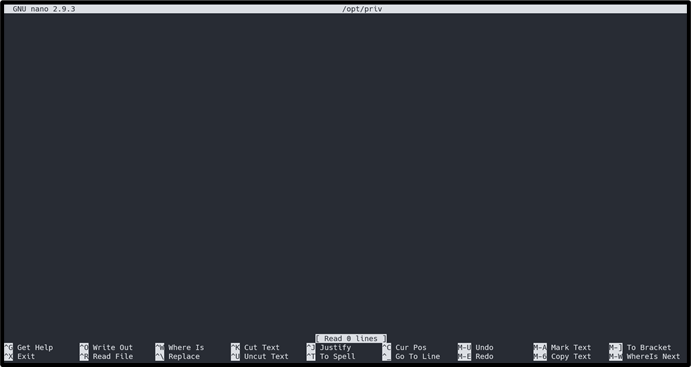
\includegraphics[width=0.99\textwidth]{imagenes/espop.png}
    \caption{Escalamiento de privilegios en OpenAdmin}
\end{figure}
Buscando información sobre escalamiento de privilegios mediante nano se encuentra que se puede obtener una Shell para ejecutar comandos como root utilizando la combinación de opciones “Ctrl+R” y “Ctrl+X” para ejecutar comando. El comando por ingresar será “reset; sh 1\textgreater\&0 2\textgreater\&0”, con el que se consigue una Shell.
\begin{figure}[H]
    \centering
    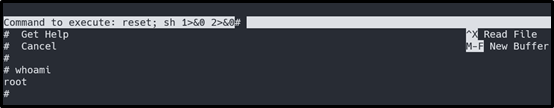
\includegraphics[width=0.99\textwidth]{imagenes/acroot.png}
    \caption{Acceso al usuario root en OpenAdmin}
\end{figure}
Una vez que se tiene la Shell, se procede a verificar que somos el usuario “root” como se indica en la imagen anterior.
\clearpage
\subsubsection{Post-explotación}
En la parte de post-explotación se procede a extraer los hashes pertenecientes a los usuarios del sistema.
\begin{figure}[H]
    \centering
    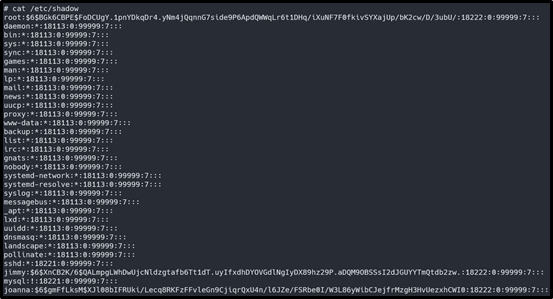
\includegraphics[width=0.99\textwidth]{imagenes/hashop.png}
    \caption{Contraseñas en formato hash de OpenAdmin}
\end{figure}
\subsubsection{Recomendaciones de mitigación}
Las recomendaciones para evitar ataques mediante las vulnerabilidades y debilidades encontradas en la maquina OpenAdmin son las siguientes.
\begin{itemize}
    \item Cambiar el uso del Software OpenAdmin a uno con mayor frecuencia de actualizaciones, debido a que la versión usada en esta máquina es la última, y no recibe actualizaciones desde junio del 2018.
    \item Realizar un control en cuanto a los permisos de ejecución privilegiados permitidos a un usuario y que pueda ocasionar el escalamiento de privilegios en el sistema.
\end{itemize}